\section{Présentation de la solution spécifique}
La solution proposée s’appuie sur les services existants et vise à valoriser ces derniers. 
En effet, l’un des points fort de cette solution est de ne pas totalement bouleverser l’organisation actuelle afin de facilité sa mise en place.
Toutefois, afin de limiter les coûts logistiques, quatre sites régionaux sont créés. Ils sont pilotés par un site central sur lequel le service achat et le nouveau service location travaillent en étroite collaboration. Chacun des sites (secondaires ou non) dispose de son propre parc matériel et magasin de pièces de rechange. Des ressources assurant la maintenance sont également affectées à chacune des antennes régionales. 
Il est important de préciser que la location du matériel reste une source de revenue secondaire, en effet, la priorité est donnée aux chantiers dont GSTP est propriétaire.
D’autre part des efforts conséquents sont réalisés en ce qui concerne l’informatisation du système complet :
    \begin{itemize}
        \item les sites et les chantiers sont équipés,
        \item un intranet est mis en place et une application spécifique est développée.
    \end{itemize}

En ce qui concerne l’application, l’un des atouts d’une solution spécifique est sa capacité d’adaptation aux besoins de GSTP. 
Ainsi, les modules planification/gestion du matériel, suivi des chantiers, achat/location, facturation et gestion des stocks optimisent les activités de la direction matérielle de GSTP et visent à répondre aux attentes des futurs utilisateurs.

En conclusion, la solution présentée ne remet pas totalement en cause l’organisation actuelle, optimise les coûts logistiques et facilite l’échange d’informations entre les différents services, les sites et les chantiers. 
De plus, le découpage de GSTP en sites régionaux permettra à la société de s’imposer comme un acteur local majeur.


\section{Plan de mise en oeuvre}
    
        \paragraph{Phase 1}
        \begin{itemize}
			\item Élaboration de la solution (9 mois)
				\subitem Etude Détaillée (1 mois)
				\subitem Développement de l’application spécifique (7 mois)
				\subitem Test (1 mois)
			\item Réorganisation de GSTP (9 mois)
				\subitem Achat des sous-sites
				\subitem Affectation des nouvelles ressources
				\subitem Achat/Affectation du matériel et des pièces de rechange
				\subitem Informatisation progressive des sites et chantiers
	    \end{itemize}

		\paragraph{Phase 2}
		\begin{itemize} 
			\item Déploiement architecture technique (2 mois)
				\subitem Achat des nouveaux matériels informatiques
				\subitem Installation du réseau
				\subitem Déploiement de l'application (sites et chantiers)
		\end{itemize}

		\paragraph{Phase 3}
		\begin{itemize} 
			\item Accompagnement au changement (2 mois)
				\subitem Formation
		\end{itemize}

		\paragraph{Phase 4}
		\begin{itemize} 
			\item Déploiement (1 mois)
				\subitem Migration des données existantes
				\subitem Qualification
				\subitem Mise en production
		\end{itemize}

		\paragraph{Phase 5}
		\begin{itemize} 
			\item Support et maintenance (contractuel  2 ans)
				\subitem Support téléphonique
				\subitem Suivi et Maintenance
		\end{itemize}

    \begin{itemize}        
        \item Total (parallélisme)
    \end{itemize}

\section{Évaluation des coûts}

    \subsection{Évaluation financière}
    
        L'évaluation financière est détaillé dans l'annexe Évaluation des scénarios, ci-dessous un tableau récapitulatif.
        (Tous les prix sont indiqué HT)
    
        \subsubsection{Site central}
            \begin{tabular*}{\textwidth}{ l @{\extracolsep{\fill}} r }
	            serveur d'application principal   & 8 000€ \\ 
	            serveur de données principal      & 8 000€ $\times$ 2 \\ 
	            serveur de réseau privé virtuel   & 0€ (solution logicielle gratuite)\\ 
                firewall                          & 800€ \\ 
	            routeur                           & 500€ \\ 
	            switch                            & 200€ \\ 
	            poste client                      & 300€ $\times$ 71\\
	            imprimante                        & 200€ $\times$ 16\\ \hline
	            Sous total                        & 50 000€
            \end{tabular*}
            
        \subsubsection{Site générique}
            \begin{tabular*}{\textwidth}{ l @{\extracolsep{\fill}} r }
	            serveur d'application / données par site  & 2 000€ \\ 
	            client de réseau privé virtuel par site   & 0€ (solution logicielle gratuite)\\ 
                firewall par site                         & 800€ \\ 
	            routeur par site                          & 500€ \\ 
	            switch                                    & 200€ \\ 
	            postes clients                            & 300€ $\times$ 3 \\
	            imprimantes                               & 200€ $\times$ 3 \\ \hline
	            Sous total par site                       & 5 000€
            \end{tabular*}

        \subsubsection{Chantiers}
            \begin{tabular*}{\textwidth}{ l @{\extracolsep{\fill}} r }
	            serveur d'application / données mobile par chantier     & 2000€ \\ 
	            client de réseau privé virtuel par chanter              & 0€ (solution logicielle gratuite)\\ 
	            firewall par chantier                                   & 800€ \\ 
	            routeur par chantier                                    & 500€ \\ 
	            switch                                                  & 200€ \\ 
	            borne relais wifi de secours par chantier               & 100€ \\ 
	            smartphone par chantier                                 & 2 $\times$ 70€ + 2 $\times$ 30€ \/ mois\\ 
	            poste client                                            & 500€ $\times$ 1 \\
	            imprimante                                              & 200€ $\times$ 1 \\ \hline
	            Sous total par chantier                                 & 4 440€ + 600€ \/mois
            \end{tabular*}

-------------------------------------------------------------------------------------------------------------------------> (ADRIEN)

\section{Chiffrage de l'investissement nécessaire au déploiement des sites secondaires}

    Nous avons évalué la superficie de terrain nécessaire à chaque site secondaire entre 1500 et 2500 m². Le prix d'achat d'un tel terrain pour chaque site étant à priori trop élevé pour GSTP, nous envisageons de louer ces terrains, pour un prix moyen de 30.000€ par an.

    \subsection{immobilier}

        Concernant le matériel présent sur chaque site, il sera le même pour tous : 
        \begin{description}
	        \item[bureaux : ] Afin d'équiper les sites, au moins 8 à 10 bureaux devront être installés dans chaque site. Le prix total par site pour cet équipement s'élèvera donc à 3000€ par site (estimation pour l'installation de 10 bureaux)
	        \item[Autres coût :]  On estime à 1500€ les coûts d'équipement secondaires de chaque site (fournitures de bureau, autres mobiliers...)
        \end{description}

        \subsection{Frais Logistiques}
        Les sites secondaires étant répartis dans toute la France, leurs distance avec les différents chantiers qu'ils doivent alimenter sera inférieure à 200km.

        La mise en place de ces sites secondaires engendrera directement des couts logistiques liés aux flux physiques (matériels, matières, transports, emballages, stocks..), nous estimons ces coûts à 20 000€.

        La somme totale des dépenses liées à la mise en place de ces sites est de 32 000€ (plus 120 000€/an).

        -------------------------------------------------------------------------------------------------------------------------> (THANH)

        \subsubsection{Développement Spécifique}
        \paragraph{Objectif}

        Dans le cadre du projet GSTP, il faut maintenant évaluer les couts de développement spécifiques afin d'aider les clients à choisir une solution.

        \paragraph{Méthode}

        Étant donné que nous optons seulement pour le ``logiciels libres/open sources", le calcul ne sera basé que sur le charge de travail.\\

        On a décidé de le développement ne se sera effectué que par nos équipes sans rien externaliser.

        L’unité de calcul sera le ``jour-etude-homme'' (JEH) qui nous permettra également de rester cohérent dans le contexte du projet et de rendre plus flexible la répartition du travail. "Un jour-etude-homme" correspondra à 400 €.

    \subsection{Estimation}

    \subsubsection{Développement}
    La démarche utilisée pour le développement sera le cycle en V. 

    \begin{enumerate}
    \item \textbf{Elaboration:}\\ Il commencera par l'analyse de besoins, faisabilité et la spécification ensemble. Cette tâche nécessitera  60 jeh. \\

    En suite c'est la phase de spécification détaillée pour chaque module. Nous estimons cette phase en jeh pour chaque module à :
         - Planification : 20
         - Suivi de chantiers : 20 
         - Achat/Location : 20 
         - Fracturation : 10
         - Gestion de stocks : 10 
         - TOTAL : 90.

    \item \textbf{Construction}\\
    Une fois la spécification est établie, il faut travailler sur la conception ensemble qui prendra 30jeh. 

    \begin{center} 
        \begin{tabular}{ |c| c| c | c | c |c |}
        \hline
	    Module&Conception&Codage&Doc&Teste&Total\\ \hline
        Planification & 50 & 90 & 15 &35&190\\ \hline
        Suivi Chantier &35&90&10&25&160 \\ \hline
        Achat/Location &20&40&5&20&85  \\ \hline
        Fracturation &25&30&5&15&75\\ \hline
        Gestion de stock &30&35&5&20&90 \\
        \hline
        \end{tabular}
    \end{center}

    Les test d'intégration nécessiteront 80jeh.

    Il faut donc 775jeh pour cette phase de construction et validation.

    \subsubsection{Déploiement}

    Le déploiement se passera en général relativement vite avec la même équipe de développent. Il prendra environ 60 j*h.

    Le budget du projet s'élève à 442 000€(1015jeh).

    Il faudra 9 mois pour réaliser le projet et environ 6 personnes dans l'équipe dont le chef de projet, il exercera le suivi du projet et participera aux différentes phases de l'étude. Nous avons fait le maximum pour réduire les délais, en supposant que le chef de projet pourra effectuer parallèlement son suivi et ses tâches sur le projet. Le projet sera piloté par notre chef de projet le plus expérimenté.

    \subsubsection{Maintenance}

    Nos équipes assureront également la maintenance corrective de l'application durant 2ans, il faudra par la suite mettre en place un nouveau contrat de maintenance qui coutera 24 000€ / an. Ce contrat implique la correction de 10 bogues mineurs et de 2 bogues majeurs au maximum. Les maintenances évolutives engendreront d'autres dépenses. Mais un budget annuel de 24 000€ devrait couvrir les besoins de maintenance de GSTP.

    Sinon GSTP devra peut être embauché un nouvel employé (voir 2) ayant des compétences dans les technologies du projet afin d'assurer la maintenance (évolutive, corrective.). Son salaire sera environ 40000€ \ an.\\

    Le coût total de maintenance est très difficile à calculer à priori. 
    Par contre, par expérience le coût annuel peut être approximé à  10 \% du coût initial. Mais cela couterait trop cher à GSTP, donc la société mettra
    en place l'ensemble des actions nécessaires à réduire au maximum la maintenance de cette solution.

    \subsubsection{Formation}
        La mise en place d'une solution spécifique nécessite une connaissance solide des futurs utilisateurs, il faut concevoir et réaliser l'application afin que les futurs utilisateurs puissent se l'approprier, l'appropriation se fera également grâce aux formations
          La formation est donc une étape indispensable. Les utilisateurs ciblés sont les administratifs, les responsables et les techniciens. (il n'est pas nécessaire de former les ouvriers).\\

    Les manuels utilisateur sont créés durant la phase de développement au fur et à mesure.\\

    Pour ne pas trop impacter sur le rythme de travail des employés, il y aura environ 15 personnes par groupe de formation sachant qu'il y a 100 personnes à former  environ, il y aura environ 5 formations par groupe soit 35 formations en tout.
    Nous estimons la journée de formation à 2jeh (2 formateurs de nos équipes). Nous proposons énormément de formations afin que les employés puissent être rapidement opérationnelles et qu'ils s'adaptent vite à leur environnement de travail. Pour certains il s'agira d'un réel changement donc ces formations sont vraiment justifiées.

    Les dépenses liées aux formations sont de 70 jeh (environ 28 000€).
     

    \end{enumerate}

    \subsection{Coût total de la solution spécifique}

    Le prix total de l'investissement pour la mise en place, la formation et la maintenance pour la solution spécifique est : 783 400€.
          - Dépenses informatiques : 135 500€
          - Prix de l'aménagement des sites secondaires : 12 000€
          - Prix de la logistique nécessaire pour les sites secondaires : 20 000€
          - Location du terrain pour les sites secondaires : 120 000€
          - Coût développement spécifique : 442 000€
          - Formations : 28 000€
          - Maintenance : 24 000€

    En plus il y aura des dépenses annuelles :
          - Maintenance abonnement? : 2400€
          - Location du terrain pour les sites secondaires : 120 000€
          - Maintenance : 24 000€

        \subsection{Délai}

              D'après le plan de mise en œuvre, le temps total estimé pour la solution spécifique est de 12 mois en considérant le parallélisme de certaines phases. On va faire en même temps : l'installation des nouveaux entrepôts régionaux et l'acquisition du matériel pour la nouvelle architecture matérielle; les tests, la validation du nouveau système et la formation du personnel.

-------------------------------------------------------------------------------------------------------------------------> (BAPTISTE)

\section{Gains et ROI}
\subsection{Evaluation des gains}

    \begin{tabular}{|p{7cm}|p{5cm}|p{2cm}|}    \hline
Axe d'amélioration & Apports & Gains sur une année\\ \hline

Efficacité générale
                                  & \begin{itemize}
                                      \item Moins d'erreurs humaines
                                      \item Rapide exécution des processus
                                     \end{itemize}
                                                          & 20000€  \\ \cline{1-2}
Limiter le nombre de fournisseurs 
                                  & \begin{itemize}
                                      \item fidélisation
                                      \item réduction
                                     \end{itemize}
                                                          & 10000€  \\ \cline{1-2}
Informatiser le département matériel 
                                  & réduction du papier (5 ramettes par jour sur un an)
                                                          & 4400€  \\ \cline{1-2}
Créer 4 petits sites positionnés (en plus du site central). Sur ces sites, il y aura : un dépôt de gros matériel, un magasin de
pièces de rechange et un atelier de maintenance. 
                                  & réelles économies logistiques
                                                          & 65000€  \\ \cline{1-2}
Optimiser le service location 
                                  & Augmentation de l'exploitation du matériel
                                                          &  36000€ \\ \cline{1-2}  
Utiliser des outils d'aide à la décision
                                  & Ciblage des achats
                                                          &  36000€ \\ \cline{1-2} 
Etablir un historique des besoins en pièces de rechange
                                  & Limitations des coûts de stock et du temps de livraison des fournisseurs
                                                          &  43500€ \\ \cline{1-2} 
Effectuer des statistiques sur les pannes les plus régulières (gamme standards)
                                  & Efficacité des maintenances préventives augmentée
                                                          &   14700€\\ \cline{1-2}         
Etablir des types de panne pour les opérations de maintenance
                                  & Réduction du temps de maintenance
                                                          &   18600€\\ \cline{1-2}

Etablir des statistiques d'exploitation des machines
                                  & Réduction des coûts liés au matériel
                                                          &  31000€ \\ \hline  
\multicolumn{2}{|r|}{TOTAL :} & 279 200€ \\ \hline                                                                                                                                                                                                                      
      
\end{tabular}
        
\subsection{Calcul du ROI}

Le coût total de la solution spécifique est environ de : 783 400€ pour la première année et après pour chaque année 146 400€ dépenses supplémentaires. Le gain est estimé à 219 200€ /an. L'équation à résoudre pour obtenir le nombre
d'années après lequel on aura retour sur investissement est : (783 400- 279 200) + (nbAnnées - 1)*( 146 400 - 279 200) = 0

Après le calcul on obtient que le retour sur investissement se fera au bout de 4 ans et 10 mois.


-------------------------------------------------------------------------------------------------------------------------> (CHAFIK)
\section{Evaluation risques solutions | delaid es satisfaction utilisateur | Maintenance Compétences externes}

\section{Evaluation des risques}

\paragraph{Risque de non respect des délais\\}
C'est le risque le plus critique lors du déploiement de notre solution. Il peut être du à une mauvaise planification ou simplement au non respect des échéances de livraison de la part de nos fournisseurs. Les différentes phases de développement sont très souvent difficiles à estimer en termes de temps.
La formation associée à notre solution peut également causer d'importants retards, ainsi que le déploiement même et la mise en place de notre solution, aussi bien l'installation matérielle que logicielle.

\subparagraph{Solutions\\}
Optimiser la planification et assurer un suivi régulier pour garantir un respect des délais plus efficace. S'orienter vers des fournisseurs et des entreprises proposant un service de qualité.

\paragraph{Risque lié à la formation du personnel\\}
Le personnel de GSTP n'étant pas très à l'aise avec l'outil informatique. Le risque de difficulté d'adaptation à notre solution est important. Le passage d'un mode opératoire dépourvu d'informatique à une solution complètement automatisée peut nécessiter une formation d'une durée plus importante que celle prévue et une intervention fréquente d'un informaticien externe.

\subparagraph{Solutions\\}
Prévoir des sessions de formation de niveaux différents s'adaptant à tous les profils. Insister sur l'aspect ergonomique et la simplicité d'utilisation
de notre solution. Nommer un responsable informatique au sein des membres de GSTP et le former efficacement afin qu'il puisse intervenir sur place de manière rapide et sure en cas de problème.


\paragraph{Risque de dépassement budgétaire\\}
Une mauvaise estimation des couts peut induire un dépassement budgétaire non négligeable. Ce dépassement est une conséquence directe du non respect des échéances.

\subparagraph{Solutions\\}
Voir risque de non respect des délais.

\paragraph{Risque lié à la maintenance\\}
La maintenance représente un enjeu économique considérable pour notre société. Un mauvais déploiement de la solution peut affecter l'image de notre entreprise si bien que GSTP pourrait se tourner vers d'autres entreprises pour les opérations de maintenance.

\subparagraph{Solutions\\}
Respecter les délais lors du déploiement de la solution. Proposer des formules pour la maintenance et assurer leurs opérations dans des délais relativement courts.

\paragraph{Risque lié à l'évolution des besoins de GSTP\\}
Ce risque est étroitement lié à celui de la maintenance. L'évolutivité de certains besoins n'ayant pas été précisé par GSTP lors des phases précédentes. Un risque d'incompatibilité de la solution et des besoins évolutifs doit être pris en considération.

\subparagraph{Solutions\\}
Proposer une solution la plus générique possible. 

\section{Annexes}
    \subsection{Evaluation Scenarios}
        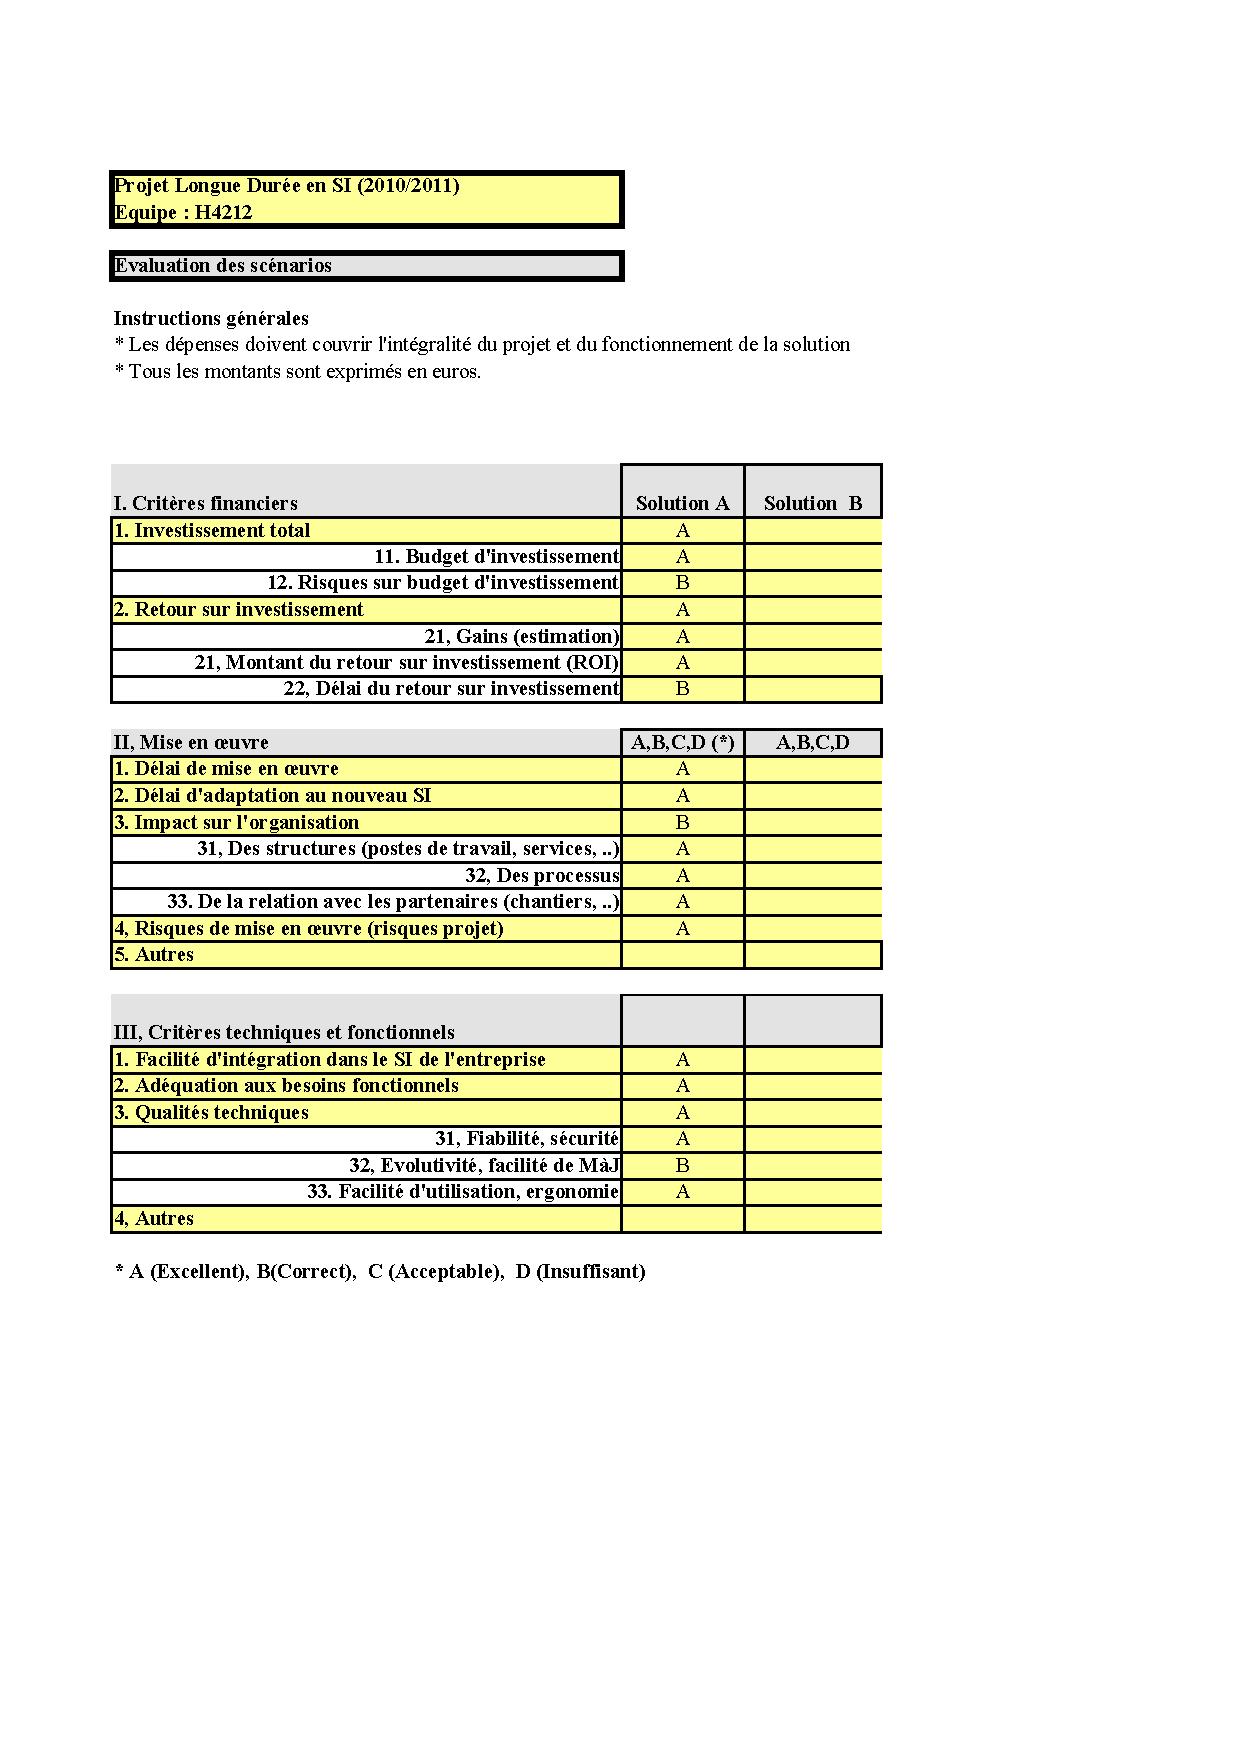
\includepdf{res/Tableau_evaluation_scenarios_PLD.pdf}

